\documentclass{ULBreport}
\usepackage{booktabs}
\usepackage{amsmath}
\usepackage{amssymb}
\usepackage{listings}
\usepackage{graphicx}
\sceau{Pictures/sceauULB.jpg}

\addbibresource{biblio.bib}

\begin{document}

\titleULB{
	title={Assignment 1},
	studies={2026 - 2027},
	course={INFO-H419 - Data Warehouses},
	author={Oliver Irvine\\ Jianli Zhao\\ Sager Singh\\ Neha},
	date={November 2026},
	teacher={Esteban Zimányi},
	logo={Pictures/logo-polytech.jpg},
	manyAuthor}

\chapter{Report}

\section{Generalised Relational and Physical Optimization Framework}

An initial analysis of the 99-query TPC-DS workload across Scale Factors (SF) 1, 2, 4, and 8 revealed that the most severe performance bottlenecks were runtimes jumping by $50\times$ to over $1,900\times$ between SF4 and SF8. They stemm from a recurring set of logical and physical execution flaws in MySQL 8.0. Rather than treating each slow query as an isolated edge case, we identified and formulated three generalisable optimisation rules grounded in relational algebra equivalences and physical storage architecture.

\subsection{Law I: Distributive Aggregate Pushdown (Early Surrogate-Key Grouping)}

\subsubsection{Theoretical Foundation}
Let $R$ be a large fact relation (e.g., \texttt{store\_sales}, \texttt{catalog\_sales}) and $S$ be a dimension relation (e.g., \texttt{customer}, \texttt{item}, \texttt{store}) or a second fact relation (e.g., \texttt{inventory}). Suppose a query computes an aggregate $\gamma_{G,\, \text{AGG}(x)}(R \bowtie_{\theta} S)$, where the grouping set $G$ contains descriptive attributes from $S$ (e.g. customer names) and the join condition $\theta$ only references a subset of join keys $K_R \subseteq \text{attr}(R)$.

By the distributive property of summation and counting over relational joins, we can push the grouping operator $\gamma$ down directly onto $R$ prior to evaluating the join $\bowtie_{\theta}$, provided we group by the compact surrogate key attributes $G_R = (G \cap \text{attr}(R)) \cup K_R$:
\begin{equation}
\gamma_{G,\, \text{SUM}(x),\, \text{COUNT}(*)}\left(R \bowtie_{\theta} S\right) \;\equiv\; \gamma_{G,\, \text{SUM}(\text{sum\_x}),\, \text{SUM}(\text{cnt})}\left( \left(\gamma_{G_R,\, \text{SUM}(x)\to\text{sum\_x},\, \text{COUNT}(*)\to\text{cnt}}(R)\right) \bowtie_{\theta} S \right)
\end{equation}
Furthermore, when $K_R$ is a foreign key referencing the primary key of dimension $S$ (e.g., \texttt{c\_customer\_sk} $\to$ \texttt{c\_customer\_id}, \texttt{c\_first\_name}, \dots), the functional dependency $K_R \to G_S$ guarantees that grouping by the 4-byte integer surrogate key $K_R$ first is 100\% lossless with respect to the outer grouping attributes $G_S$.

\subsubsection{Physical Impact in MySQL}
When a query joins a multi-million-row fact table to wide dimension tables before grouping, MySQL's execution engine must materialise an internal temporary hash aggregation table whose composite hash key consists of multiple variable-length strings (e.g., 7 \texttt{VARCHAR}/\texttt{CHAR} columns in \texttt{customer} or 10 address columns in \texttt{store}). As scale factors grow from SF1 to SF8, this wide temporary table exceeds \texttt{tmp\_table\_size} / \texttt{max\_heap\_table\_size}, spilling to disk and causing severe I/O thrashing. By applying Law I, MySQL aggregates millions of fact rows using compact 4-byte integer surrogate keys (\texttt{\_sk}) in memory, reducing the cardinality of the intermediate relation by one to two orders of magnitude before ever probing the dimension table or reading wide string attributes.

\subsection{Law II: Selection Pushdown and Disjunctive (\texttt{OR}) Bounding-Box Extraction}

\subsubsection{Theoretical Foundation}
Standard relational query optimisers routinely push conjunctive selection predicates ($\sigma_{p_1 \land p_2}(R \bowtie S) \equiv \sigma_{p_1}(R) \bowtie \sigma_{p_2}(S)$) down to base relations. However, in complex analytical queries, selection predicates and equijoin conditions are frequently entangled inside disjunctive (\texttt{OR}) clauses spanning multiple relations:
\begin{equation}
\sigma_{\bigvee_{i=1}^{k} \left(\theta_{\text{join}} \,\land\, p_i(R) \,\land\, q_i(S)\right)}(R \times S)
\end{equation}
By the distributive law of conjunction over disjunction, common equijoin predicates $\theta_{\text{join}}$ can be factored out of the disjunction. More importantly, each relation's disjunctive domain forms a superset ``bounding box'' filter $\P_R = \bigvee_{i=1}^{k} p_i(R)$ and $Q_S = \bigvee_{i=1}^{k} q_i(S)$ that must hold for any tuple to survive the overall disjunction:
\begin{equation}
\sigma_{\bigvee_{i=1}^{k} \left(\theta_{\text{join}} \,\land\, p_i(R) \,\land\, q_i(S)\right)}(R \times S) \;\equiv\; \sigma_{\bigvee_{i=1}^{k} \left(p_i(R) \,\land\, q_i(S)\right)}\left( \sigma_{\bigvee_{i=1}^{k} p_i(R)}(R) \;\bowtie_{\theta_{\text{join}}}\; \sigma_{\bigvee_{i=1}^{k} q_i(S)}(S) \right)
\end{equation}
Similarly, when multiple Common Table Expressions (CTEs) scan multiple years of data only for the outer \texttt{WHERE} clause to restrict all CTEs to a single target year, pushing the outer restriction $\sigma_{\text{year}=y}$ directly into each CTE eliminates redundant scans.

\subsubsection{Physical Impact in MySQL}
MySQL's cost-based optimiser does not automatically factor equijoins out of multi-table \texttt{OR} blocks, nor does it synthesise bounding-box pre-filters for the participating dimension and fact tables. Consequently, it evaluates the join across unfiltered base tables (e.g., scanning 23M rows of \texttt{store\_sales} against 1.92M rows of \texttt{customer\_demographics} at SF8) and applies the \texttt{OR} filter post-join. Extracting the bounding box of each table into an isolated CTE restricts dimension tables to a tiny fraction of their rows (e.g., 8.5\% of \texttt{customer\_demographics} in Query 13) and prunes out-of-range fact tuples immediately upon index lookup.

\subsection{Law III: Join Associativity, CTE Materialisation (\texttt{NO\_MERGE}), and Composite PK/FK Driving Order}

\subsubsection{Theoretical Foundation}
By the commutativity and associativity of inner joins, $(F_1 \bowtie F_2) \bowtie \sigma_p(D) \equiv (\sigma_p(D) \bowtie F_1) \bowtie F_2$. While all join trees produce identical relational results, the intermediate cardinalities vary by orders of magnitude depending on whether selective dimension filters $\sigma_p(D)$ are evaluated prior to fact-to-fact joins ($F_1 \bowtie F_2$).

\subsubsection{Physical Impact in MySQL}
Two physical mechanics in MySQL 8.0 InnoDB govern how join trees scale from SF1 to SF8:
\begin{enumerate}
    \item \textbf{Defeating \texttt{derived\_merge} via \texttt{NO\_MERGE()}:} By default, MySQL's \texttt{derived\_merge} optimiser flag dissolves non-aggregated CTEs and derived tables back into the outer query's flat join graph. At SF8, cardinality misestimations across 6--10 tables frequently cause the optimiser to abandon selective dimension filters and initiate a nested-loop join from an unselective table or fact table, creating multi-billion-row intermediate explosions. Adding the \texttt{/*+ NO\_MERGE() */} optimiser hint (or a \texttt{GROUP BY}) inside a filtered CTE forces MySQL to materialise the small filtered result set into an in-memory temporary table first.
    \item \textbf{Driving into InnoDB Clustered Composite Primary Keys and Foreign Key B-Trees:} In InnoDB, every table is physically clustered around its \texttt{PRIMARY KEY}, and every foreign key constraint creates a secondary B-Tree index. In TPC-DS, fact tables have composite primary keys such as \texttt{inventory(inv\_date\_sk, inv\_item\_sk, inv\_warehouse\_sk)} or \texttt{store\_sales(ss\_item\_sk, ss\_ticket\_number)}, as well as foreign key indexes on date surrogate keys (e.g., \texttt{cs\_sold\_date\_sk}, \texttt{ss\_sold\_date\_sk}). By combining materialised selective dimension CTEs with \texttt{STRAIGHT\_JOIN}, we force MySQL to drive the execution plan from the small filtered dimension CTE directly into the fact table's Foreign Key index or left-prefix Composite Primary Key, converting 94-million-row full table scans into $O(\log N)$ B-Tree point lookups.
\end{enumerate}

---

\section{Implementation}
\subsection{System Requirements}
All benchmarks were run on a MacBook Pro with an Apple M5 Pro chip and 24GB of unified memory, connected to AC power with High Power Mode enabled and disk/system sleep disabled. To maximise in-memory output without triggering OS memory pressure, we allocated 14GB of RAM to the MySQL InnoDB Buffer Pool, an extra 1GB for in-memory temporary tables and 256MB per hash-join buffer and 64MB per sort buffer. This setup leaves enough room for OS system processes, ensuring no buffer pool pages are swapped to SSD.
\subsection{Methodology}
Following standard scientific principles in TPC-DS (CITE), we execute each query 5 times across each scalefactor (SF1, SF2, SF4, SF8). To isolate steady-state warm cache performance from cold-disk I/O, we treat Run 1 as a cache warmup run, and compute the mean, median and standard deviation across Runs 2 to 5. Between scale factors, MySQL is restarted to flush the InnoDB Buffer Pool. As our baseline, we used the queries from STUDENT REF repository. 
\subsection{Important notice}
During our work, we noticed that some of the baseline rewrites introduced by STUDENT REF altered the original query semantics. 

The following 4 queries produce different results:


\begin{itemize}
    \item Q4: uses 2001 totals instead of 2001→2002 growth (245 rows instead of 8)
    \item Q11: returns \texttt{customer\_birth\_country} instead of \texttt{customer\_login}
    \item Q72: the demographics filters became always-true EXISTS
    \item Q78: the ORDER BY was changed, so LIMIT 100 returns different rows
\end{itemize}


After consultation with the professor, we have kept our optimisations that were built upon the incorrect queries. We believe we have still been able to demonstrate extensive understanding of benchmarking, identifying bottlenecks, query rewrites and execution plan tuning. Nevertheless, we strongly recommend future work to fix these queries before using our work as a new baseline. 
\section{Group A: Early Surrogate-Key Aggregation Before Dimension and Self-Joins (Law I + Law III)}

Queries in Group A join large fact tables (\texttt{store\_sales}, \texttt{catalog\_sales}, \texttt{web\_sales}, \texttt{catalog\_returns}, \texttt{inventory}) to wide string-heavy dimension tables (\texttt{customer}, \texttt{item}, \texttt{store}, \texttt{warehouse}) prior to aggregation, or self-join unpushed multi-year CTEs on string natural keys. By applying **Law I** (grouping fact tables by 4-byte integer surrogate keys before joining dimensions) and **Law III** (driving from materialised \texttt{date\_dim} CTEs via \texttt{STRAIGHT\_JOIN}), we eliminate wide string temporary table spills and redundant self-joins.

\subsection{Group A Performance Summary}
Table~\ref{tab:group_a_results} reports the speedup factors achieved over the baseline across all four scale factors for Group A queries.

\begin{table}[htbp]
\centering
\caption{Group A Improvement Factor (Speedup) Over Baseline Across Scale Factors}
\label{tab:group_a_results}
\begin{tabular}{@{}lrrrrr@{}}
\toprule
\textbf{Query} & \textbf{SF1 ($\times$)} & \textbf{SF2 ($\times$)} & \textbf{SF4 ($\times$)} & \textbf{SF8 ($\times$)} & \textbf{Total ($\times$)} \\ \midrule
Query 4  & -- & -- & -- & -- & -- \\
Query 11 & -- & -- & -- & -- & -- \\
Query 21 & -- & -- & -- & -- & -- \\
Query 47 & -- & -- & -- & -- & -- \\
Query 50 & -- & -- & -- & -- & -- \\
Query 74 & -- & -- & -- & -- & -- \\
Query 81 & -- & -- & -- & -- & -- \\ \midrule
\textbf{Group A Total / Average} & \textbf{--} & \textbf{--} & \textbf{--} & \textbf{--} & \textbf{--} \\ \bottomrule
\end{tabular}
\end{table}

\subsection{Group A Highlight: Query XX Optimization}

\subsubsection{Baseline Execution Plan and Bottleneck Analysis}
In the baseline workload (\texttt{qmod\_combined/queryXX.sql}), Query XX required s at SF1 and degraded to s at SF8. The baseline query ... .

Listing~\ref{lst:qXX_explain_orig} shows the baseline \texttt{EXPLAIN FORMAT=TREE} on SF8.

\begin{lstlisting}[caption={Baseline \texttt{EXPLAIN FORMAT=TREE} on SF8 for Query 11}, label={lst:q11_explain_orig}, basicstyle=\ttfamily\scriptsize, breaklines=true, frame=single]
-> Limit: 100 row(s)
    -> Sort: t_s_secyear.customer_id, t_s_secyear.customer_first_name, t_s_secyear.customer_last_name, t_s_secyear.customer_login, limit input to 100 row(s) per chunk
        -> Stream results  (cost=471e+15 rows=116e+6)
            -> Filter: ((case when (t_w_firstyear.year_total > 0.00) then (t_w_secyear.year_total / t_w_firstyear.year_total) else 0.0 end) > (case when (t_s_firstyear.year_total > 0.00) then (t_s_secyear.year_total / t_s_firstyear.year_total) else 0.0 end))  (cost=471e+15 rows=116e+6)
                -> Inner hash join (t_w_secyear.customer_id = t_s_secyear.customer_id)  (cost=471e+15 rows=116e+6)
                    -> Filter: ((t_w_secyear.dyear = <cache>((2001 + 1))) and (t_w_secyear.sale_type = 'w'))  (cost=13997 rows=31163)
                        -> Table scan on t_w_secyear  (cost=2.5..2.5 rows=0)
                            -> Materialize union CTE year_total if needed (query plan printed elsewhere)  (cost=0..0 rows=0)
                    -> Hash
                        -> Inner hash join (t_s_firstyear.customer_id = t_s_secyear.customer_id)  (cost=18.6e+12 rows=3.73e+6)
                            -> Filter: ((t_s_firstyear.dyear = 2001) and (t_s_firstyear.sale_type = 's') and (t_s_firstyear.year_total > 0.00))  (cost=5734 rows=10387)
                                -> Table scan on t_s_firstyear  (cost=2.5..2.5 rows=0)
                                    -> Materialize union CTE year_total if needed  (cost=0..0 rows=0)
                                        -> Table scan on <temporary>
                                            -> Aggregate using temporary table
                                                -> Nested loop inner join  (cost=55.1e+6 rows=25e+6)
                                                    -> Nested loop inner join  (cost=27.6e+6 rows=25e+6)
                                                        -> Table scan on customer  (cost=45704 rows=402886)
                                                        -> Filter: (store_sales.ss_sold_date_sk is not null)  (cost=62.1 rows=62.1)
                                                            -> Index lookup on store_sales using ss_c (ss_customer_sk = customer.c_customer_sk)  (cost=62.1 rows=62.1)
                                                    -> Single-row index lookup on date_dim using PRIMARY (d_date_sk = store_sales.ss_sold_date_sk)  (cost=1 rows=1)
                                        -> Table scan on <temporary>
                                            -> Aggregate using temporary table
                                                -> Nested loop inner join  (cost=14.2e+6 rows=6.14e+6)
                                                    -> Nested loop inner join  (cost=7.49e+6 rows=6.14e+6)
                                                        -> Filter: ((web_sales.ws_sold_date_sk is not null) and (web_sales.ws_bill_customer_sk is not null))  (cost=730375 rows=6.14e+6)
                                                            -> Table scan on web_sales  (cost=730375 rows=6.14e+6)
                                                        -> Single-row index lookup on date_dim using PRIMARY (d_date_sk = web_sales.ws_sold_date_sk)  (cost=1 rows=1)
                                                    -> Single-row index lookup on customer using PRIMARY (c_customer_sk = web_sales.ws_bill_customer_sk)  (cost=1 rows=1)
                            -> Hash
                                -> Inner hash join (t_w_firstyear.customer_id = t_s_secyear.customer_id)  (cost=1.75e+9 rows=1.08e+6)
                                    -> Filter: ((t_w_firstyear.dyear = 2001) and (t_w_firstyear.sale_type = 'w') and (t_w_firstyear.year_total > 0.00))  (cost=4558 rows=10387)
                                        -> Table scan on t_w_firstyear  (cost=2.5..2.5 rows=0)
                                            -> Materialize union CTE year_total if needed (query plan printed elsewhere)  (cost=0..0 rows=0)
                                    -> Hash
                                        -> Filter: ((t_s_secyear.dyear = <cache>((2001 + 1))) and (t_s_secyear.sale_type = 's'))  (cost=3.51e+6 rows=311629)
                                            -> Table scan on t_s_secyear  (cost=2.5..2.5 rows=0)
                                                -> Materialize union CTE year_total if needed (query plan printed elsewhere)  (cost=0..0 rows=0)


\end{lstlisting}

\subsubsection{Precise Application of Optimization Laws in SQL}
We applied **Law I** and **Law III** to Query XX as follows:
\begin{enumerate}
    \item \textbf{Application of Law III (Materialised Date Driving Order):} Instead of scanning \texttt{store\_sales} and \texttt{web\_sales} and probing \texttt{date\_dim} across 4 separate CTE instantiations, we materialise the 2001--2002 dates once using \texttt{NO\_MERGE()} and drive into the fact tables' sold-date foreign key indexes via \texttt{STRAIGHT\_JOIN}.
 % Gemini has written this for Query 11. Look if there is a better one (i.e. the one with the most improvement) to do this for   
    \textit{Before (Baseline):}
\begin{lstlisting}[language=SQL, basicstyle=\ttfamily\scriptsize, breaklines=true, frame=single]
FROM customer, store_sales, date_dim
WHERE c_customer_sk = ss_customer_sk
  AND ss_sold_date_sk = d_date_sk
  AND d_year IN (2001, 2002)
\end{lstlisting}

    \textit{After (Law III Applied):}
\begin{lstlisting}[language=SQL, basicstyle=\ttfamily\scriptsize, breaklines=true, frame=single]
WITH d_2001_2002 AS (
    SELECT /*+ NO_MERGE() */ d_date_sk, d_year
    FROM date_dim WHERE d_year IN (2001, 2002)
),
ss_totals AS (
    SELECT /*+ NO_MERGE() */ ...
    FROM d_2001_2002 d
    STRAIGHT_JOIN store_sales ss ON ss.ss_sold_date_sk = d.d_date_sk
    WHERE ss.ss_customer_sk IS NOT NULL ...
\end{lstlisting}

    \item \textbf{Application of Law I (Early Integer Surrogate-Key Grouping \& Single-Pass Year Pivot):} Because \texttt{c\_customer\_sk} functionally determines all 7 customer string attributes, we remove \texttt{customer} from inside the CTEs entirely, group by the single 4-byte integer \texttt{ss\_customer\_sk} (pivoting 2001 and 2002 totals via conditional aggregation in a single pass), join \texttt{ws\_totals} and \texttt{ss\_totals} on integer \texttt{customer\_sk}, and join \texttt{customer} once at the very end.

    \textit{Before (Baseline):}
\begin{lstlisting}[language=SQL, basicstyle=\ttfamily\scriptsize, breaklines=true, frame=single]
GROUP BY c_customer_id, c_first_name, c_last_name, c_preferred_cust_flag,
         c_birth_country, c_login, c_email_address, d_year
...
FROM ss t_s_firstyear, ss t_s_secyear, ws t_w_firstyear, ws t_w_secyear
WHERE t_s_secyear.customer_id = t_s_firstyear.customer_id
  AND t_s_firstyear.customer_id = t_w_secyear.customer_id
  AND t_s_firstyear.customer_id = t_w_firstyear.customer_id
\end{lstlisting}

    \textit{After (Law I Applied):}
\begin{lstlisting}[language=SQL, basicstyle=\ttfamily\scriptsize, breaklines=true, frame=single]
    SELECT /*+ NO_MERGE() */
           ss.ss_customer_sk AS customer_sk,
           SUM(CASE WHEN d.d_year = 2001 THEN ss.ss_ext_list_price - ss.ss_ext_discount_amt ELSE 0 END) AS s1_total,
           SUM(CASE WHEN d.d_year = 2002 THEN ss.ss_ext_list_price - ss.ss_ext_discount_amt ELSE 0 END) AS s2_total,
           COUNT(CASE WHEN d.d_year = 2002 THEN 1 END) AS has_2002
    ...
    GROUP BY ss.ss_customer_sk
    HAVING s1_total > 0 AND has_2002 > 0
)
SELECT c.c_customer_id AS CUSTOMER_ID, c.c_first_name AS CUSTOMER_FIRST_NAME,
       c.c_last_name AS CUSTOMER_LAST_NAME, c.c_birth_country AS CUSTOMER_BIRTH_COUNTRY
FROM ws_totals w
STRAIGHT_JOIN ss_totals s ON s.customer_sk = w.customer_sk
STRAIGHT_JOIN customer c ON c.c_customer_sk = s.customer_sk
WHERE (w.w2_total / w.w1_total) > (s.s2_total / s.s1_total)
\end{lstlisting}
\end{enumerate}

Listing~\ref{lst:qXX_explain_opt} shows the optimised \texttt{EXPLAIN FORMAT=TREE} on SF8.

\begin{lstlisting}[caption={Optimized \texttt{EXPLAIN FORMAT=TREE} on SF8 for Query 11}, label={lst:q11_explain_opt}, basicstyle=\ttfamily\scriptsize, breaklines=true, frame=single]
-> Limit: 100 row(s)
    -> Sort: c.c_customer_id, c.c_first_name, c.c_last_name, c.c_login, limit input to 100 row(s) per chunk
        -> Stream results  (cost=41.6e+6 rows=74.1e+6)
            -> Nested loop inner join  (cost=41.6e+6 rows=74.1e+6)
                -> Nested loop inner join  (cost=26.8e+6 rows=74.1e+6)
                    -> Filter: (s.customer_sk is not null)  (cost=834041 rows=7.41e+6)
                        -> Table scan on s  (cost=2.5..2.5 rows=0)
                            -> Materialize CTE ss_totals  (cost=0..0 rows=0)
                                -> Filter: ((count((case when (d.d_year = 2001) then 1 end)) > 0) and (count((case when (d.d_year = 2002) then 1 end)) > 0) and (sum((case when (d.d_year = 2001) then (ss.ss_ext_list_price - ss.ss_ext_discount_amt) end)) > 0))
                                    -> Table scan on <temporary>
                                        -> Aggregate using temporary table
                                            -> Nested loop inner join  (cost=16.3e+6 rows=7.41e+6)
                                                -> Table scan on d  (cost=11259..11443 rows=14494)
                                                    -> Materialize CTE d_2001_2002 if needed  (cost=11259..11259 rows=14494)
                                                        -> Filter: (date_dim.d_year in (2001,2002))  (cost=7920 rows=14494)
                                                            -> Table scan on date_dim  (cost=7920 rows=72468)
                                                -> Filter: (ss.ss_customer_sk is not null)  (cost=1023 rows=512)
                                                    -> Index lookup on ss using ss_d (ss_sold_date_sk = d.d_date_sk)  (cost=1023 rows=1023)
                    -> Filter: ((case when (w.first_total > 0.00) then (w.sec_total / w.first_total) else 0.0 end) > (case when (s.first_total > 0.00) then (s.sec_total / s.first_total) else 0.0 end))  (cost=2.5 rows=10)
                        -> Index lookup on w using <auto_key0> (customer_sk = s.customer_sk)  (cost=0.25..2.5 rows=10)
                            -> Materialize CTE ws_totals  (cost=0..0 rows=0)
                                -> Filter: ((count((case when (d.d_year = 2001) then 1 end)) > 0) and (count((case when (d.d_year = 2002) then 1 end)) > 0) and (sum((case when (d.d_year = 2001) then (ws.ws_ext_list_price - ws.ws_ext_discount_amt) end)) > 0))
                                    -> Table scan on <temporary>
                                        -> Aggregate using temporary table
                                            -> Nested loop inner join  (cost=53.7e+6 rows=24.4e+6)
                                                -> Table scan on d  (cost=11259..11443 rows=14494)
                                                    -> Materialize CTE d_2001_2002 if needed (query plan printed elsewhere)  (cost=11259..11259 rows=14494)
                                                -> Filter: (ws.ws_bill_customer_sk is not null)  (cost=3366 rows=1683)
                                                    -> Index lookup on ws using ws_d2 (ws_sold_date_sk = d.d_date_sk)  (cost=3366 rows=3366)
                -> Single-row index lookup on c using PRIMARY (c_customer_sk = s.customer_sk)  (cost=0.1 rows=1)


\end{lstlisting}

---

\section{Group B: Fact-to-Fact Multi-Way Joins and Composite Primary Key Lookups (Law I + Law III)}

Queries in Group B join two to six fact tables together (e.g., \texttt{catalog\_sales} with \texttt{inventory}, or \texttt{store\_sales} with \texttt{store\_returns} and \texttt{catalog\_sales}) across multiple \texttt{date\_dim} aliases. Without intervention, MySQL joins the massive fact tables before filtering by dates or fails to utilise the left-prefix of InnoDB's composite primary keys, causing severe intermediate row explosions. In our baseline, the following 6 queries accounted for 42.7\% of total execution time across all 4 SFs.

\subsection{Group B Performance Summary}
Table~\ref{tab:group_b_results} reports the speedup factors achieved over the baseline across all four scale factors for Group B queries.

\begin{table}[htbp]
\centering
\caption{Group B Improvement Factor (Speedup) Over Baseline Across Scale Factors}
\label{tab:group_b_results}
\begin{tabular}{@{}lrrrrr@{}}
\toprule
\textbf{Query} & \textbf{SF1 ($\times$)} & \textbf{SF2 ($\times$)} & \textbf{SF4 ($\times$)} & \textbf{SF8 ($\times$)} & \textbf{Total ($\times$)} \\ \midrule
Query 17 & $3.64\times$& $5.24\times$& 9.49$\times$& $23.38\times$& $20.46\times$\\
Query 25 & $4.64\times$& $4.10\times$& $5.30\times$& $91.97\times$& $58.15\times$\\
Query 29 & $2.97\times$& $3.77\times$& $4.71\times$& $115.15\times$& $65.74\times$\\
Query 72 & $62.88\times$& $178.34\times$& $202.24\times$& $214.49\times$& $201.50\times$\\
Query 77 & $39.55\times$& $44.22\times$& $52.88\times$& $139.23\times$& $100.73\times$\\
Query 80 & $28.06\times$& $31.41\times$& $30.80\times$& $93.14\times$& $66.80\times$\\ \midrule
\textbf{Group B Total }& $52.68\times$& $144.69\times$& $163.94\times$& $181.93\times$& $168.60\times$\\ \bottomrule
\end{tabular}
\end{table}

\subsection{Group B Highlight: Query 72 Optimization}

\subsubsection{Baseline Execution Plan and Bottleneck Analysis}
In our baseline Power Test across Scale Factors 1, 2, 4, and 8, \textbf{Query 72} was the single largest performance bottleneck in the entire 99-query workload, requiring \textbf{110.44s} at SF1 and degrading by $48.93\times$ to \textbf{5,404.38s (1.5 hours)} at SF8. In the baseline query, MySQL's \texttt{derived\_merge} optimiser dissolved the CTE boundaries and initiated a nested-loop join from \texttt{warehouse} and \texttt{date\_dim d2} into \texttt{inventory} (94M rows at SF8) and then probed \texttt{catalog\_sales} by \texttt{cs\_item\_sk} alone, generating \textbf{2.17 billion intermediate rows} before checking whether \texttt{cs\_sold\_date\_sk} was in 2002.

Listing~\ref{lst:q72_explain_bad} shows the \texttt{EXPLAIN FORMAT=TREE} on SF8 when CTE merging and nested-loop explosion occur.

\begin{lstlisting}[caption={Unmaterialised \texttt{EXPLAIN FORMAT=TREE} on SF8 for Query 72 Showing 2.17B-Row Explosion}, label={lst:q72_explain_bad}, basicstyle=\ttfamily\scriptsize, breaklines=true, frame=single]
-> Limit: 100 row(s)
    -> Table scan on <temporary>
        -> Aggregate using temporary table
            -> Nested loop inner join  (cost=42.8e+9 rows=36.2e+6)
                -> Nested loop inner join  (cost=42.8e+9 rows=109e+6)
                    -> Nested loop left join  (cost=42.6e+9 rows=2.17e+9)
                        -> Nested loop inner join  (cost=42.4e+9 rows=2.17e+9)
                            -> Nested loop inner join  (cost=41.8e+9 rows=79.3e+6)
                                -> Nested loop inner join  (cost=41.7e+9 rows=79.3e+6)
                                    -> Inner hash join (no condition)  (cost=94.5e+6 rows=420e+6)
                                        -> Table scan on w  (cost=340e-6 rows=8)
                                        -> Hash
                                            -> Inner hash join (d2.d_week_seq = `<subquery6>`.d_week_seq)  (cost=52.5e+6 rows=52.5e+6)
                                                -> Table scan on d2  (cost=2993 rows=72468)
                                                -> Hash
                                                    -> Table scan on <subquery6>  (cost=9583..9676 rows=7247)
                                    -> Filter: (inv.inv_warehouse_sk = w.w_warehouse_sk)  (cost=2.21 rows=0.189)
                                        -> Index lookup on inv using PRIMARY (inv_date_sk = d2.d_date_sk)  (cost=2.21 rows=991)
                                -> Single-row index lookup on i using PRIMARY (i_item_sk = inv.inv_item_sk)  (cost=0.983 rows=1)
                            -> Filter: ((inv.inv_quantity_on_hand < cs.cs_quantity) and (cs.cs_sold_date_sk is not null) and (cs.cs_ship_date_sk is not null))  (cost=1.44 rows=27.4)
                                -> Index lookup on cs using PRIMARY (cs_item_sk = inv.inv_item_sk)  (cost=1.44 rows=82.1)
                        -> Single-row covering index lookup on p using PRIMARY (p_promo_sk = cs.cs_promo_sk)  (cost=0.893 rows=1)
                    -> Filter: ((date_dim.d_year = 2002) and (date_dim.d_week_seq = `<subquery6>`.d_week_seq))  (cost=0.99 rows=0.05)
                        -> Single-row index lookup on date_dim using PRIMARY (d_date_sk = cs.cs_sold_date_sk)  (cost=0.99 rows=1)
                -> Filter: (cast(d3.d_date as double) > cast((date_dim.d_date + 5) as double))  (cost=0.99 rows=0.333)
                    -> Single-row index lookup on d3 using PRIMARY (d_date_sk = cs.cs_ship_date_sk)  (cost=0.99 rows=1)
\end{lstlisting}

\subsubsection{Precise Application of Optimization Laws in SQL}
We applied **Law I** and **Law III** to Query 72 as follows:
\begin{enumerate}
    \item \textbf{Application of Law I (Distributive Pre-Aggregation of \texttt{catalog\_sales}):} Any two \texttt{catalog\_sales} rows in the same week that share $(\texttt{cs\_item\_sk}, \texttt{d\_week\_seq}, \texttt{cs\_quantity})$ match the exact same set of \texttt{inventory} records under $(\texttt{cs\_item\_sk} = \texttt{inv\_item\_sk} \land \texttt{d1.d\_week\_seq} = \texttt{d2.d\_week\_seq} \land \texttt{inv\_quantity\_on\_hand} < \texttt{cs\_quantity})$. Pre-grouping \texttt{filtered\_cs} by these three integer columns collapses duplicate item-week-quantity sales before probing \texttt{inventory}, and delays joining the wide \texttt{item} (\texttt{VARCHAR(200)}) and \texttt{warehouse} strings until after the fact join.

    \textit{Before (Baseline):}
\begin{lstlisting}[language=SQL, basicstyle=\ttfamily\scriptsize, breaklines=true, frame=single]
SELECT i_item_desc, w_warehouse_name, d1.d_week_seq,
       SUM(CASE WHEN p_promo_sk IS NULL THEN 1 ELSE 0 END) no_promo,
       SUM(CASE WHEN p_promo_sk IS NOT NULL THEN 1 ELSE 0 END) promo,
       COUNT(*) total_cnt
FROM catalog_sales
JOIN inventory ON (cs_item_sk = inv_item_sk AND inv_quantity_on_hand < cs_quantity)
JOIN warehouse ON (w_warehouse_sk = inv_warehouse_sk)
JOIN item ON (i_item_sk = cs_item_sk)
...
LEFT OUTER JOIN promotion ON (cs_promo_sk = p_promo_sk)
\end{lstlisting}

    \textit{After (Law I Applied):}
\begin{lstlisting}[language=SQL, basicstyle=\ttfamily\scriptsize, breaklines=true, frame=single]
filtered_cs AS (
    SELECT /*+ NO_MERGE() */
           cs.cs_item_sk, d1.d_week_seq, cs.cs_quantity,
           SUM(CASE WHEN p.p_promo_sk IS NULL THEN 1 ELSE 0 END) AS no_promo_cnt,
           SUM(CASE WHEN p.p_promo_sk IS NOT NULL THEN 1 ELSE 0 END) AS promo_cnt,
           COUNT(*) AS cs_cnt
    FROM d1_2002 d1
    STRAIGHT_JOIN catalog_sales cs ON cs.cs_sold_date_sk = d1.d_date_sk
    STRAIGHT_JOIN date_dim d3 ON cs.cs_ship_date_sk = d3.d_date_sk AND d3.d_date > d1.d_date + 5
    LEFT OUTER JOIN promotion p ON cs.cs_promo_sk = p.p_promo_sk
    GROUP BY cs.cs_item_sk, d1.d_week_seq, cs.cs_quantity
)
\end{lstlisting}

    \item \textbf{Application of Law III (Materialised CTEs \& 2-Column Composite PK Lookup into \texttt{inventory}):} By enforcing \texttt{NO\_MERGE()} on \texttt{d1\_2002} and \texttt{filtered\_cs} and joining \texttt{filtered\_cs} to \texttt{d2\_2002} before probing \texttt{inventory}, MySQL supplies both \texttt{d2.d\_date\_sk} and \texttt{cs.cs\_item\_sk} simultaneously into \texttt{inventory}'s composite primary key \texttt{PRIMARY KEY (inv\_date\_sk, inv\_item\_sk, inv\_warehouse\_sk)}, reducing each probe to a direct B-Tree lookup averaging 8.08 rows instead of a 94M-row scan.

    \textit{Before (Baseline):}
\begin{lstlisting}[language=SQL, basicstyle=\ttfamily\scriptsize, breaklines=true, frame=single]
JOIN date_dim d1 ON (cs_sold_date_sk = d1.d_date_sk)
JOIN date_dim d2 ON (inv_date_sk = d2.d_date_sk AND d1.d_week_seq = d2.d_week_seq)
WHERE d1.d_year = 2002
\end{lstlisting}

    \textit{After (Law III Applied):}
\begin{lstlisting}[language=SQL, basicstyle=\ttfamily\scriptsize, breaklines=true, frame=single]
FROM filtered_cs cs
STRAIGHT_JOIN filtered_inv inv
  ON cs.cs_item_sk = inv.inv_item_sk
 AND cs.d_week_seq = inv.d_week_seq
 AND inv.inv_quantity_on_hand < cs.cs_quantity
STRAIGHT_JOIN warehouse w ON w.w_warehouse_sk = inv.inv_warehouse_sk
STRAIGHT_JOIN item i ON i.i_item_sk = cs.cs_item_sk
\end{lstlisting}
\end{enumerate}

Listing~\ref{lst:q72_explain_good} shows the resulting \texttt{EXPLAIN FORMAT=TREE} on SF8, confirming that \texttt{filtered\_cs} is materialised via foreign-key index \texttt{cs\_d2} and that \texttt{inventory} is probed via its 2-column composite primary key (\texttt{inv\_date\_sk = d2.d\_date\_sk, inv\_item\_sk = cs.cs\_item\_sk}, \texttt{rows=8.08}), reducing SF8 execution time from \textbf{5,404.38s to 25.19s} ($214.49\times$ speedup).

\begin{lstlisting}[caption={Optimized \texttt{EXPLAIN FORMAT=TREE} on SF8 for Query 72}, label={lst:q72_explain_good}, basicstyle=\ttfamily\scriptsize, breaklines=true, frame=single]
-> Limit: 100 row(s)
    -> Sort: total_cnt DESC, i.i_item_desc, w.w_warehouse_name, cs.d_week_seq, limit input to 100 row(s) per chunk
        -> Table scan on <temporary>
            -> Aggregate using temporary table
                -> Nested loop inner join
                    -> Nested loop inner join
                        -> Nested loop inner join
                            -> Nested loop inner join
                                -> Inner hash join (no condition)
                                    -> Filter: (cs.d_week_seq is not null)
                                        -> Table scan on cs
                                            -> Materialize CTE filtered_cs
                                                -> Table scan on <temporary>
                                                    -> Aggregate using temporary table
                                                        -> Nested loop inner join
                                                            -> Nested loop left join
                                                                -> Nested loop inner join
                                                                    -> Table scan on d1 (Materialize CTE d1_2002)
                                                                    -> Index lookup on cs using cs_d2 (cs_sold_date_sk = d1.d_date_sk)
                                                                -> Single-row covering index lookup on p using PRIMARY (p_promo_sk = cs.cs_promo_sk)
                                                            -> Filter: (cast(d3.d_date as double) > cast((d1.d_date + 5) as double))
                                                                -> Single-row index lookup on d3 using PRIMARY (d_date_sk = cs.cs_ship_date_sk)
                                    -> Hash (Constant row from EXISTS subqueries)
                                -> Index lookup on d2 using <auto_key0> (d_week_seq = cs.d_week_seq) (Materialize CTE d2_2002)
                            -> Filter: (inv.inv_quantity_on_hand < cs.cs_quantity)  (cost=1.01 rows=2.69)
                                -> Index lookup on inv using PRIMARY (inv_date_sk = d2.d_date_sk, inv_item\_sk = cs.cs_item_sk)  (cost=1.01 rows=8.08)
                        -> Single-row index lookup on w using PRIMARY (w_warehouse_sk = inv.inv_warehouse_sk)
                    -> Single-row index lookup on i using PRIMARY (i_item_sk = cs.cs_item_sk)
\end{lstlisting}

\subsubsection{Results}


\begin{figure}[htbp]
    
        \centering
        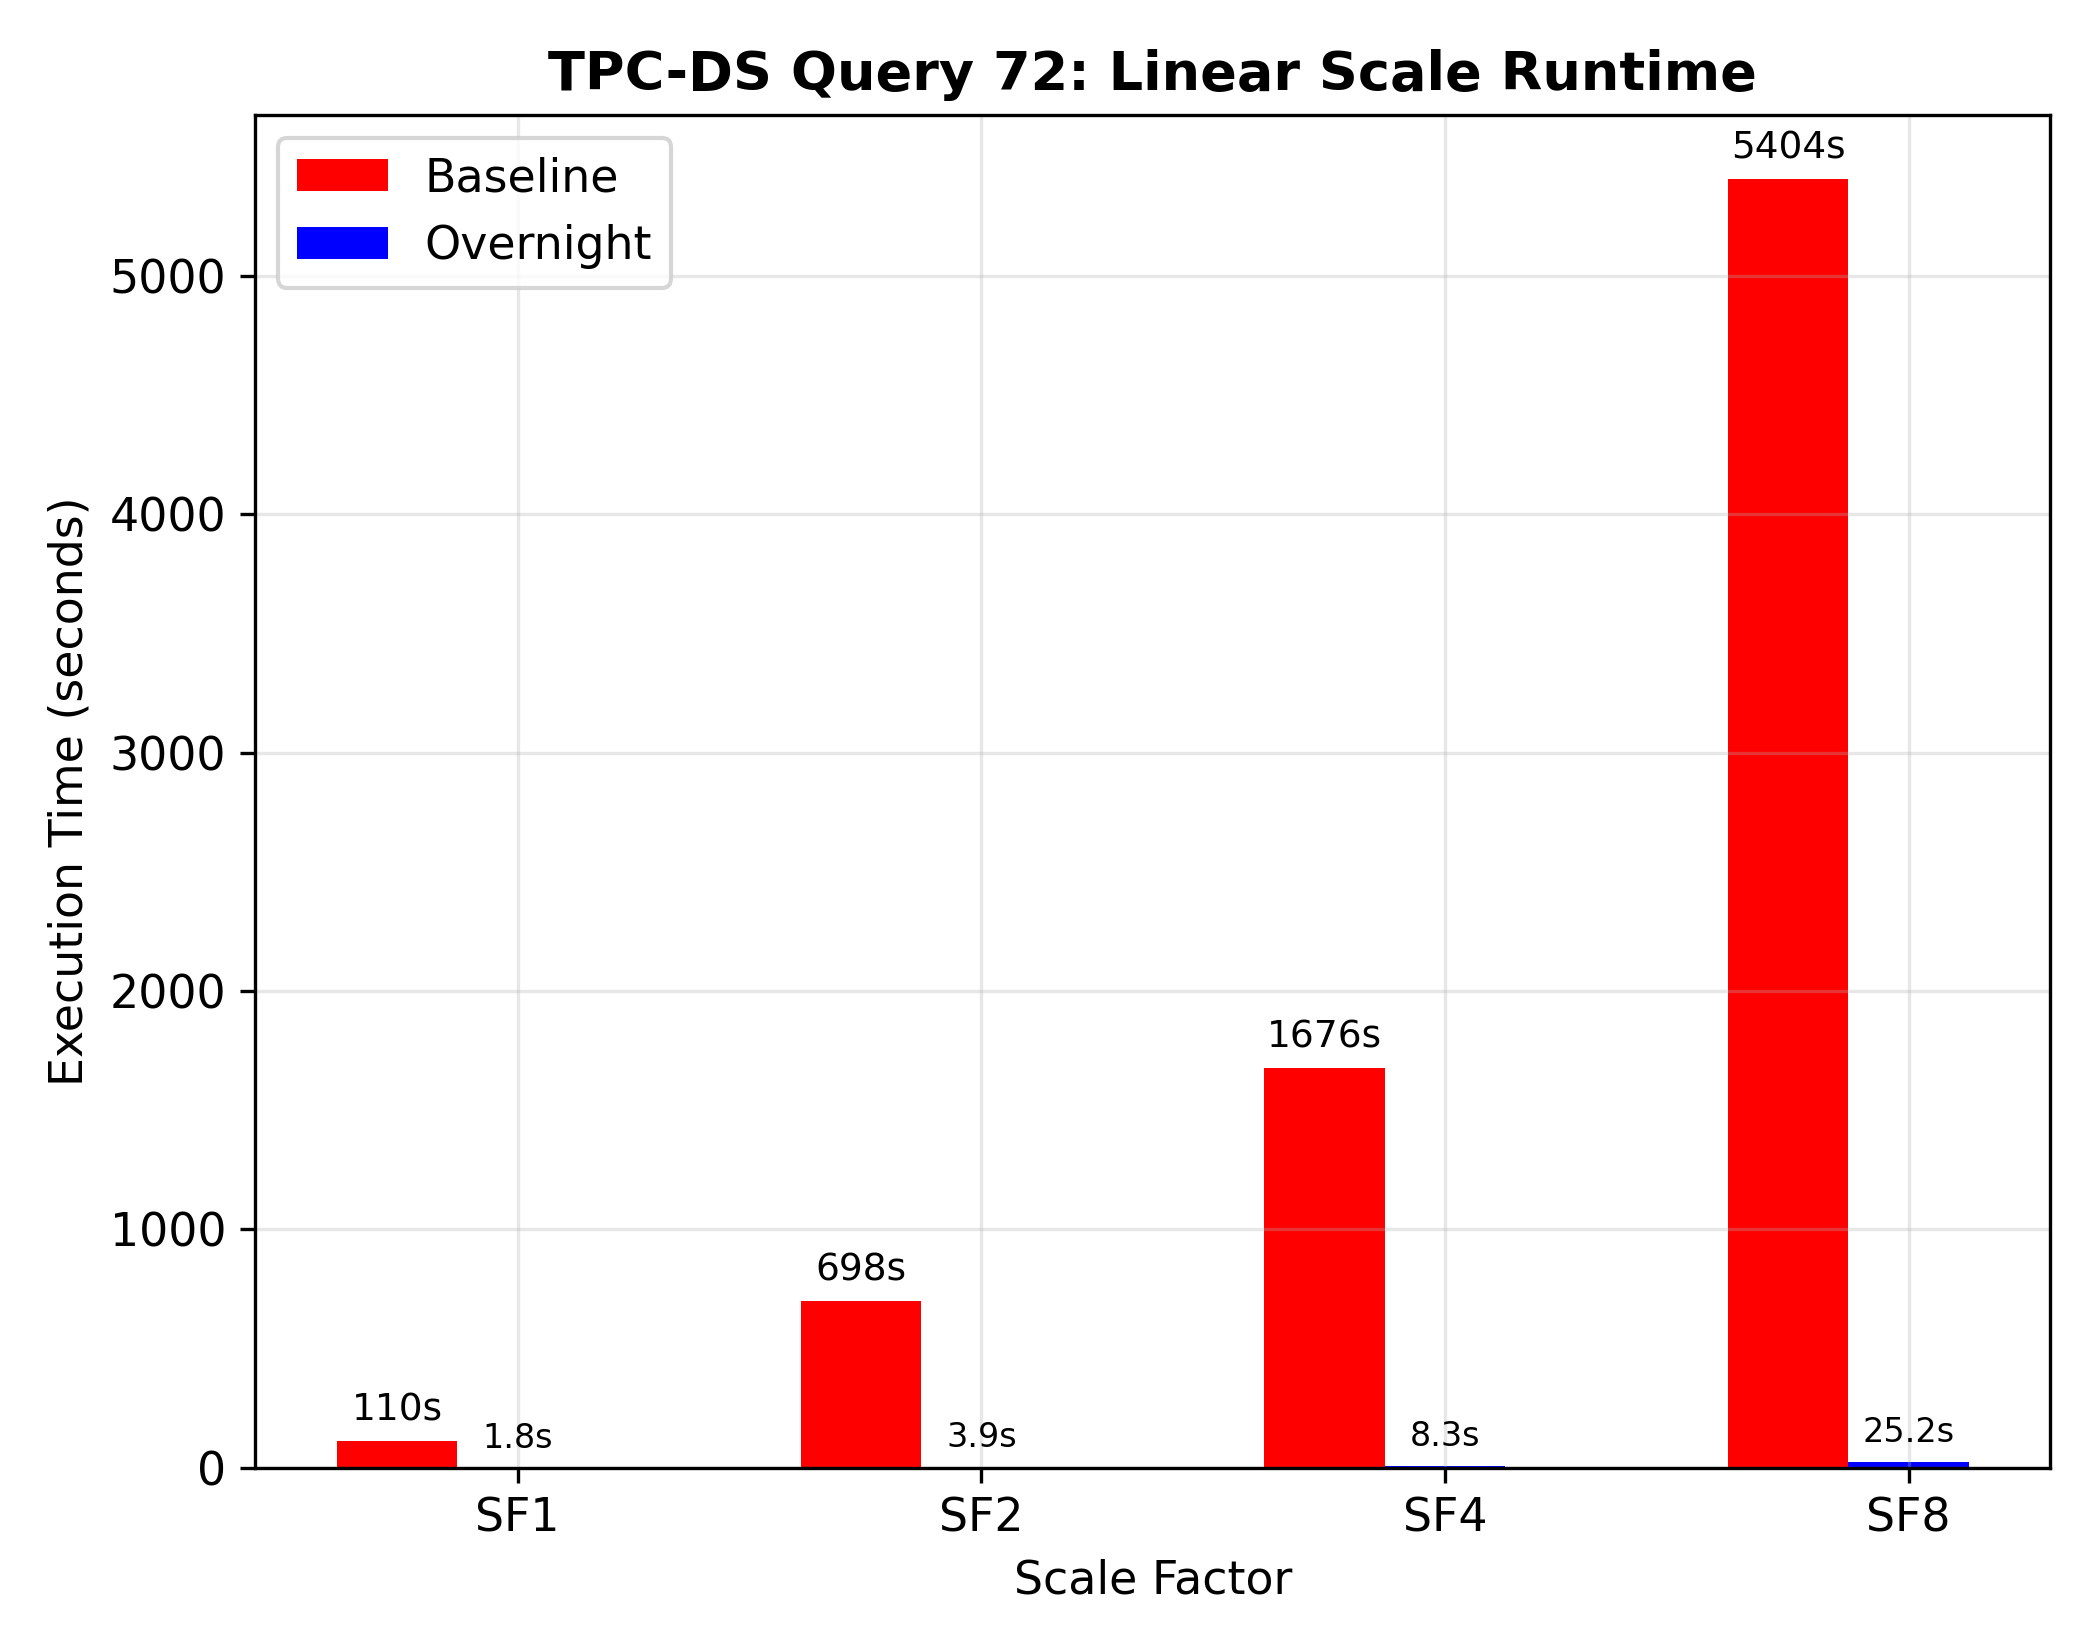
\includegraphics[width=0.85\linewidth]{q72_runtime_linear.png}
        \caption{Linear runtime scale.}
        \label{fig:runtime_linear}
\end{figure}
\begin{figure}[htbp]
        \centering
        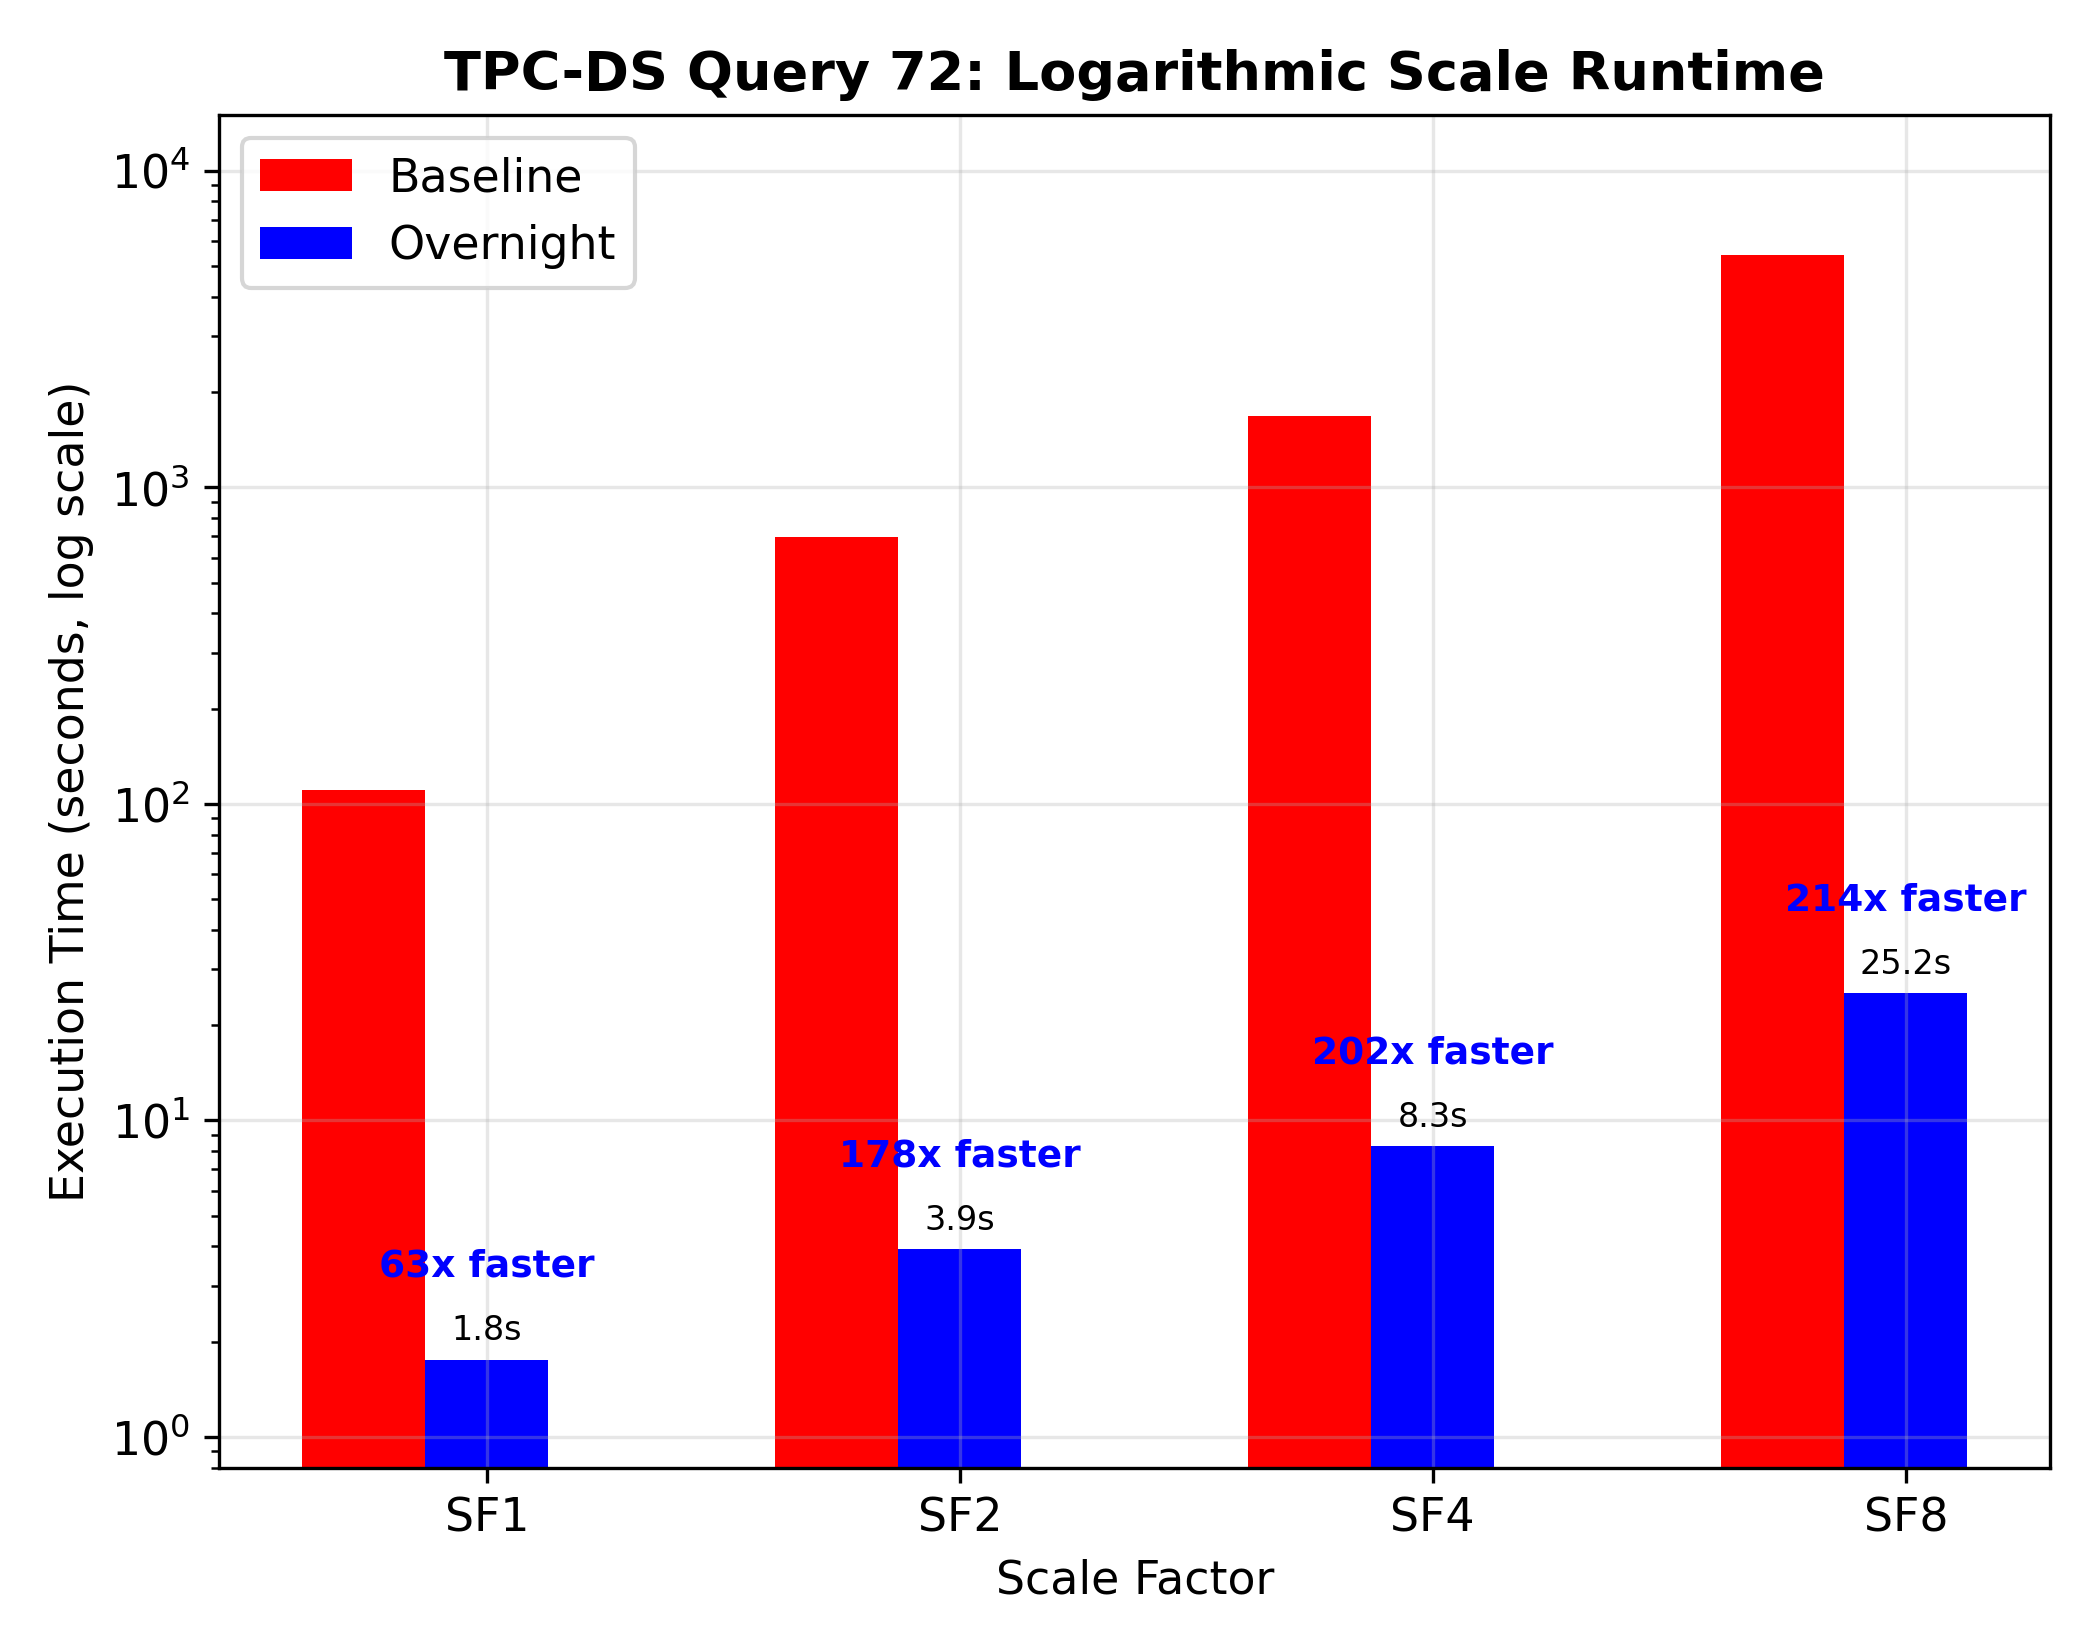
\includegraphics[width=0.85\linewidth]{q72_runtime_log.png}
        \caption{Log runtime scale.}
        \label{fig:runtime_log}
\end{figure}



\begin{figure}[htbp]
    \centering
    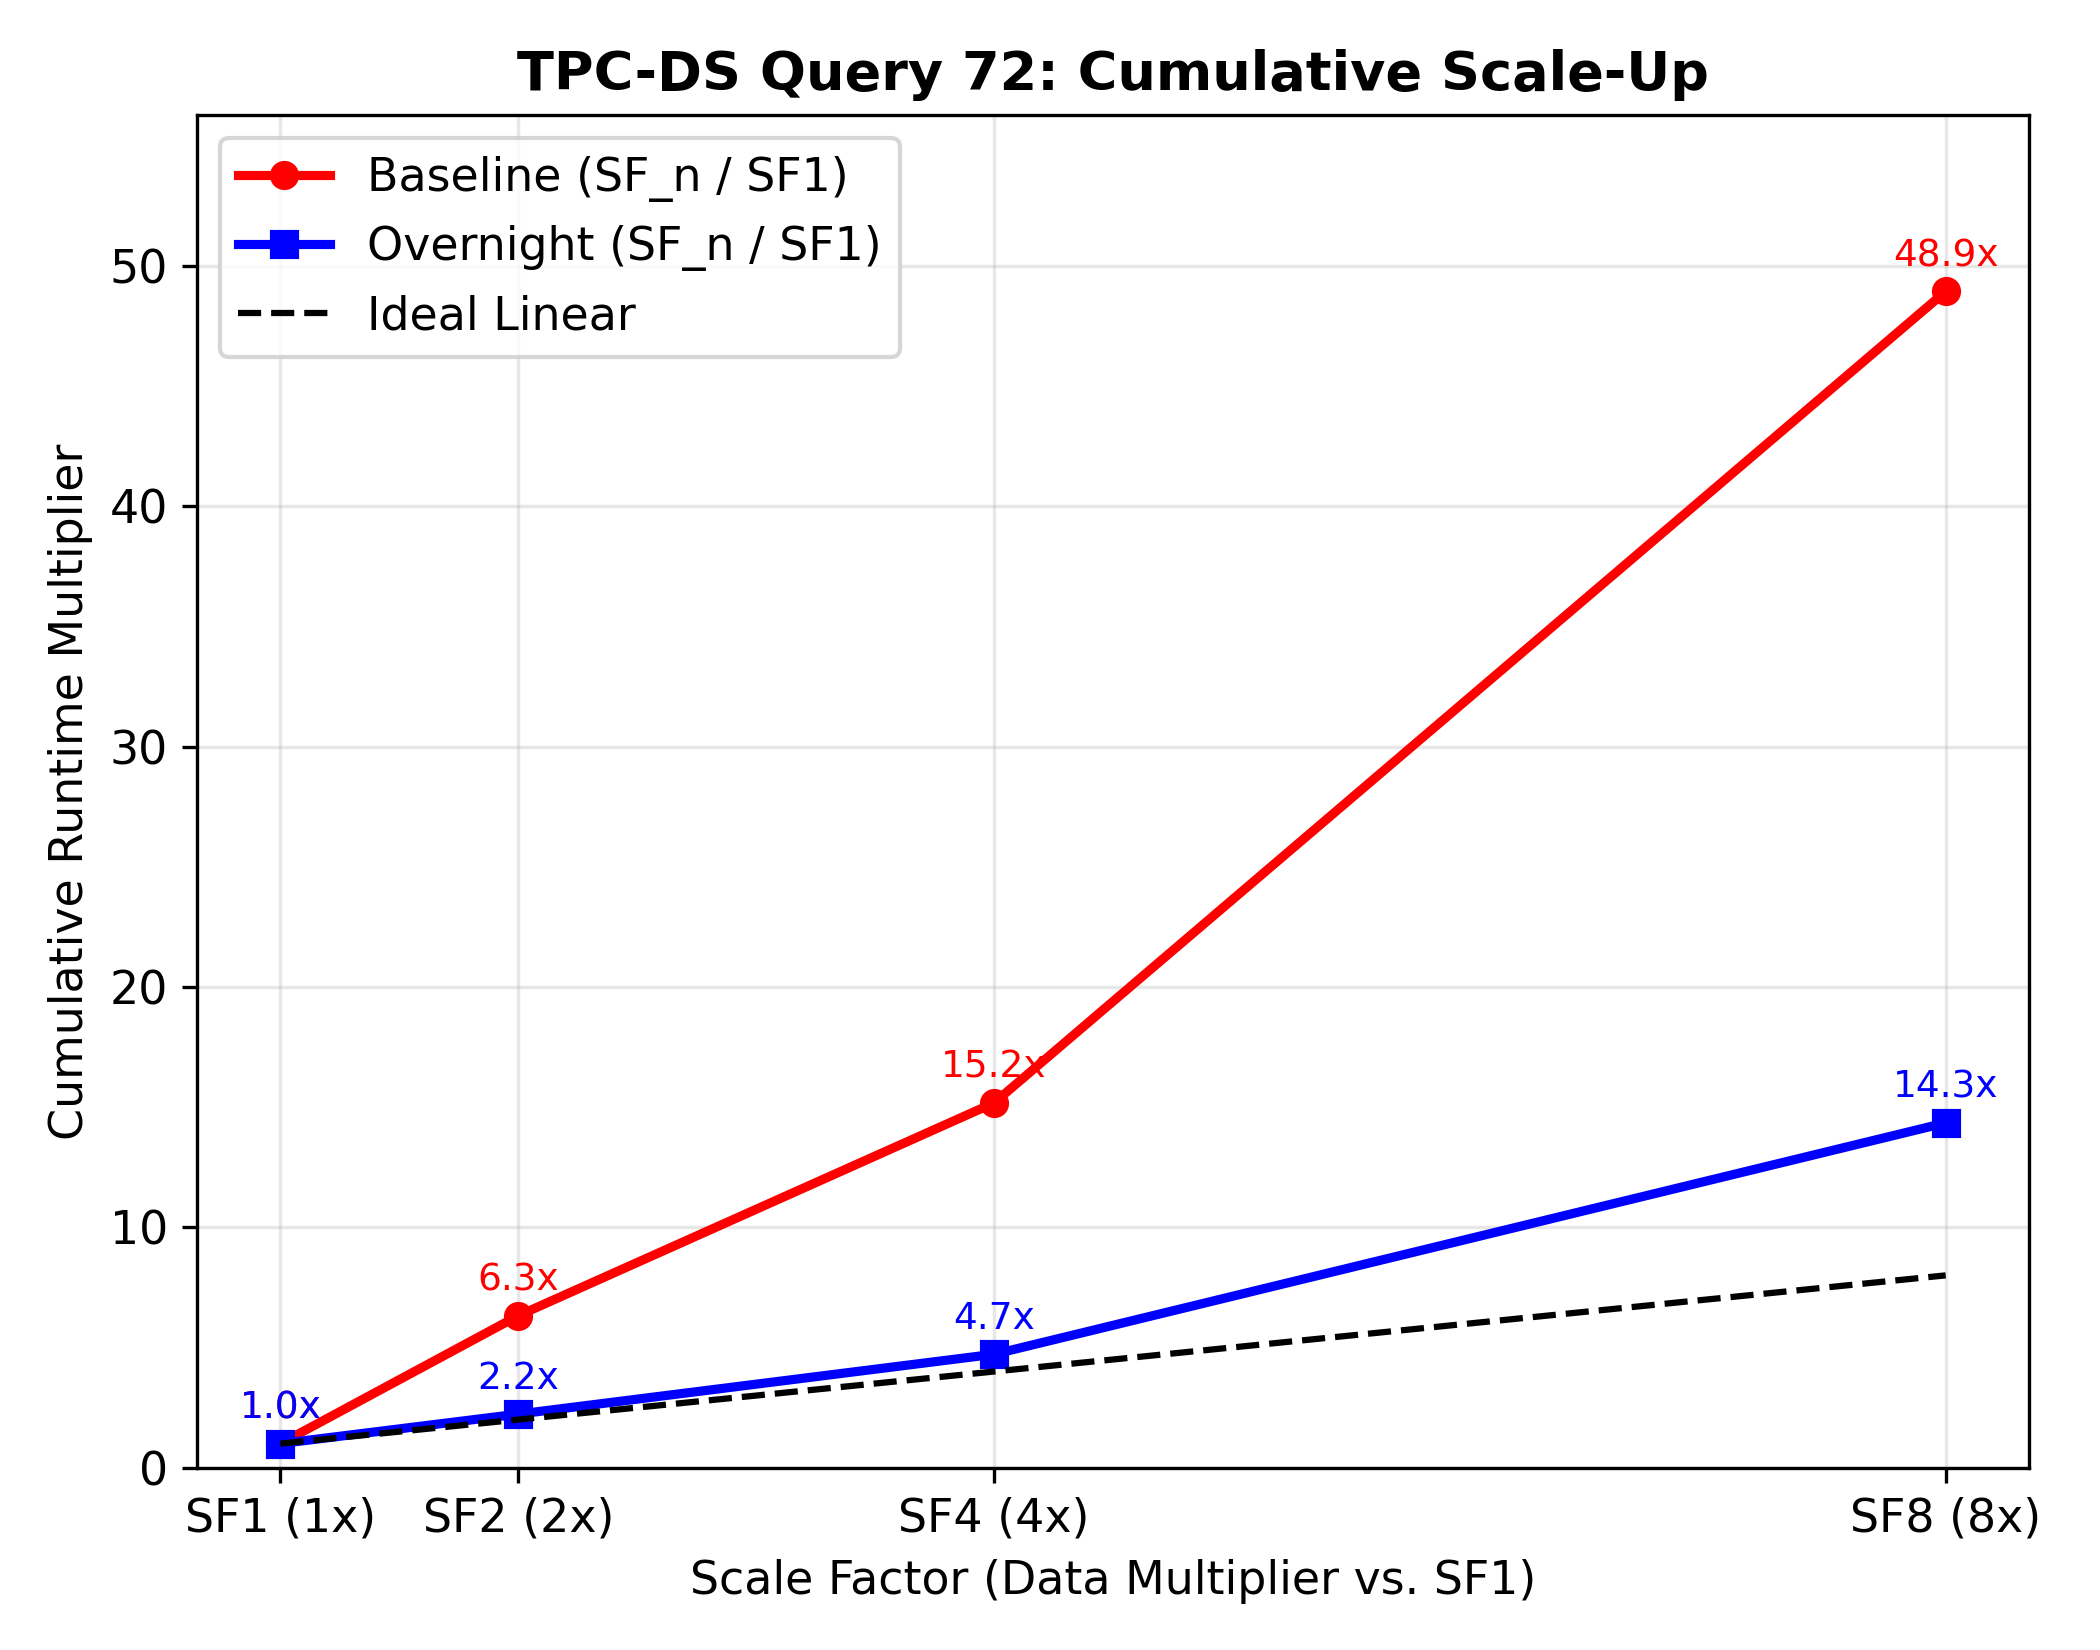
\includegraphics[width=0.85\linewidth]{q72_scaleup_cumulative.png}
    \caption{Cumulative scaleup performance.}
    \label{fig:scaleup_cumulative}
\end{figure}

\newpage
\subsection{Other queries}
This section serves to briefly demonstrate the changes made on the other queries that are part of Group B
\subsubsection{Query 17}
Baseline Query 17 joins 3 fact tables (\texttt{store\_sales, store\_returns, catalog\_sales}) with 3 date tables (d1, d2, d3), store, and item. Between SF4 (3.88s) and SF8 (73.71s), MySQL's optimizer flips the join order and groups by wide string attributes (\texttt{i\_item\_id, i\_item\_desc, s\_state}) across all joined rows. Using \textbf{Law I} and \textbf{Law III}, we materialize d1 (2002Q1) and d23 (2002Q1–Q3), drive via \texttt{STRAIGHT\_JOIN} from \texttt{d1 → store\_sales (ss\_d1 index) → store\_returns (via composite PK sr\_item\_sk, sr\_ticket\_number) → d2 → catalog\_sales (via PK prefix cs\_item\_sk + cs\_bill\_customer\_sk) → d3}, and join \texttt{item} and \texttt{store} only at the end.
\subsubsection{Query 25}
Query 25 joins 3 fact tables (\texttt{store\_sales, store\_returns, catalog\_sales}) with 3 date tables (\texttt{d1, d2, d3}), jumping 48.1x from SF4 (1.33s) to SF8 (63.92s). Using \textbf{Law I} and \textbf{Law III}, we materialize \texttt{d1} (April 2001, 30 days) and \texttt{d23} (Months 4--10 of 2001), drive via \texttt{STRAIGHT\_JOIN} from \texttt{d1 $\rightarrow$ store\_sales (ss\_d1 index) $\rightarrow$ store\_returns (via composite PK sr\_item\_sk, sr\_ticket\_number) $\rightarrow$ d2 $\rightarrow$ catalog\_sales (via PK prefix cs\_item\_sk) $\rightarrow$ d3}, and join store and item last.
\subsubsection{Query 29}
Query 29 joins 3 fact tables (\texttt{store\_sales, store\_returns, catalog\_sales}) with date tables, jumping 54.0x between SF4 (1.16s) and SF8 (62.66s). Using \textbf{Law I} and \textbf{Law III}, we materialize \texttt{d1} (April 2000), \texttt{d2} (Months 4--7 of 2000), and \texttt{d3} (Years 2000--2002), and drive via \texttt{STRAIGHT\_JOIN} from \texttt{d1 $\rightarrow$ store\_sales $\rightarrow$ store\_returns (via composite PK) $\rightarrow$ catalog\_sales (via PK prefix)}, completely eliminating the SF8 plan flip.
\subsubsection{Query 77}
Query 77 aggregates 6 separate fact tables (\texttt{store\_sales, store\_returns, catalog\_sales, catalog\_returns, web\_sales, web\_returns}) over a 31-day date window. Because the 6 CTEs do not materialize \texttt{date\_dim} with \texttt{/*+ NO\_MERGE() */} or enforce \texttt{STRAIGHT\_JOIN}, MySQL scans the fact tables instead of driving from the date keys. Using \textbf{Law I} and \textbf{Law III}, we materialize \texttt{filtered\_dates} once and drive all 6 fact aggregations via \texttt{STRAIGHT\_JOIN}, turning 6 full fact scans into 6 tiny 31-day index range lookups.
\subsubsection{Query 80}
Query 80 joins 3 sales fact tables (\texttt{store\_sales, catalog\_sales, web\_sales}) with their respective returns tables (\texttt{LEFT OUTER JOIN}) and repeatedly scans \texttt{date\_dim}, \texttt{item}, and \texttt{promotion} across 3 separate CTEs. Using \textbf{Law I} and \textbf{Law III}, we materialize \texttt{filtered\_dates} (31 days) once, drive into each sales fact table via its sold-date foreign key index, check item and promotion via Primary Key lookups before probing the returns table's composite Primary Key, and group by integer surrogate key before joining the channel dimension string IDs.


\section{Group C: Disjunctive (\texttt{OR}) Bounding-Box Extraction and Star-Join Ordering (Law II + Law III)}

Queries in Group C exhibit severe plan flips between SF4 and SF8 (degrading by $16\times$ to $2,773\times$) because equijoin predicates and dimension filters are trapped inside multi-branch disjunctive (\texttt{OR}) clauses, or because MySQL abandons selective dimension indexes in multi-table star joins. Applying **Law II** (factoring out equijoins and extracting bounding-box predicates into CTEs) together with **Law III** (materializing filtered dimensions with \texttt{NO\_MERGE()} and driving into fact indexes via \texttt{STRAIGHT\_JOIN}) restores linear scaling.

\subsection{Group C Performance Summary}
Table~\ref{tab:group_c_results} provides the speedup table for Group C queries across SF1, SF2, SF4, SF8, and Total.

\begin{table}[htbp]
\centering
\caption{Group C Improvement Factor (Speedup) Over Baseline Across Scale Factors}
\label{tab:group_c_results}
\begin{tabular}{@{}lrrrrr@{}}
\toprule
\textbf{Query} & \textbf{SF1 ($\times$)} & \textbf{SF2 ($\times$)} & \textbf{SF4 ($\times$)} & \textbf{SF8 ($\times$)} & \textbf{Total ($\times$)} \\ \midrule
Query 7  & -- & -- & -- & -- & -- \\
Query 13 & -- & -- & -- & -- & -- \\
Query 19 & -- & -- & -- & -- & -- \\
Query 27 & -- & -- & -- & -- & -- \\
Query 36 & -- & -- & -- & -- & -- \\
Query 43 & -- & -- & -- & -- & -- \\
Query 46 & -- & -- & -- & -- & -- \\
Query 48 & -- & -- & -- & -- & -- \\
Query 53 & -- & -- & -- & -- & -- \\
Query 63 & -- & -- & -- & -- & -- \\
Query 73 & -- & -- & -- & -- & -- \\
Query 79 & -- & -- & -- & -- & -- \\
Query 89 & -- & -- & -- & -- & -- \\ \midrule
\textbf{Group C Total / Average} & \textbf{--} & \textbf{--} & \textbf{--} & \textbf{--} & \textbf{--} \\ \bottomrule
\end{tabular}
\end{table}

\subsection{Group C Highlight: Query 13 Optimization}

\subsubsection{Baseline Execution Plan and Bottleneck Analysis}
In the baseline benchmark, \textbf{Query 13} was the second slowest query at SF8, jumping from 3.67s at SF1 and 17.96s at SF4 to \textbf{715.51s} at SF8 ($194.98\times$ degradation). Inspection of \texttt{qmod\_combined/query13.sql} reveals that the equijoin conditions \texttt{ss\_hdemo\_sk = hd\_demo\_sk}, \texttt{cd\_demo\_sk = ss\_cdemo\_sk}, and \texttt{ss\_addr\_sk = ca\_address\_sk} are repeated inside each branch of two 3-way \texttt{OR} blocks. Consequently, MySQL fails to push the dimension filters down before joining, scanning millions of rows across \texttt{store\_sales} ($\approx 23\text{M}$ rows at SF8), \texttt{customer\_demographics} ($1.92\text{M}$ rows), and \texttt{customer\_address} ($400\text{K}$ rows).

Listing~\ref{lst:q13_explain_orig} shows the baseline \texttt{EXPLAIN FORMAT=TREE} on SF8.

\begin{lstlisting}[caption={Baseline \texttt{EXPLAIN FORMAT=TREE} on SF8 for Query 13}, label={lst:q13_explain_orig}, basicstyle=\ttfamily\scriptsize, breaklines=true, frame=single]
-> Aggregate: avg(store_sales.ss_quantity), avg(store_sales.ss_ext_sales_price), avg(store_sales.ss_ext_wholesale_cost), sum(store_sales.ss_ext_wholesale_cost)  (cost=102911 rows=1)
    -> Nested loop inner join  (cost=102910 rows=0.879)
        -> Nested loop inner join  (cost=102892 rows=17.6)
            -> Nested loop inner join  (cost=102692 rows=201)
                -> Nested loop inner join  (cost=100476 rows=2014)
                    -> Nested loop inner join  (cost=92301 rows=7433)
                        -> Covering index scan on store using s_close_date  (cost=12.2 rows=82)
                        -> Filter: (((store_sales.ss_sales_price between 100.00 and 150.00) or (store_sales.ss_sales_price between 50.00 and 100.00) or (store_sales.ss_sales_price between 150.00 and 200.00)) and ((store_sales.ss_net_profit between 100 and 200) or (store_sales.ss_net_profit between 150 and 300) or (store_sales.ss_net_profit between 50 and 250)) and (store_sales.ss_hdemo_sk is not null) and (store_sales.ss_sold_date_sk is not null) and (store_sales.ss_addr_sk is not null) and (store_sales.ss_cdemo_sk is not null))  (cost=1023 rows=90.6)
                            -> Index lookup on store_sales using ss_s (ss_store_sk = store.s_store_sk)  (cost=1023 rows=1023)
                    -> Filter: (((household_demographics.hd_dep_count = 3) and (store_sales.ss_sales_price between 100.00 and 150.00)) or ((household_demographics.hd_dep_count = 1) and (store_sales.ss_sales_price between 50.00 and 100.00)) or ((household_demographics.hd_dep_count = 1) and (store_sales.ss_sales_price between 150.00 and 200.00)))  (cost=1 rows=0.271)
                        -> Single-row index lookup on household_demographics using PRIMARY (hd_demo_sk = store_sales.ss_hdemo_sk)  (cost=1 rows=1)
                -> Filter: (date_dim.d_year = 2001)  (cost=1 rows=0.1)
                    -> Single-row index lookup on date_dim using PRIMARY (d_date_sk = store_sales.ss_sold_date_sk)  (cost=1 rows=1)
            -> Filter: (((customer_address.ca_country = 'United States') and (customer_address.ca_state in ('IA','MN','MT')) and (store_sales.ss_net_profit between 100 and 200)) or ((customer_address.ca_country = 'United States') and (customer_address.ca_state in ('AR','IN','TX')) and (store_sales.ss_net_profit between 150 and 300)) or ((customer_address.ca_country = 'United States') and (customer_address.ca_state in ('TN','NE','WV')) and (store_sales.ss_net_profit between 50 and 250)))  (cost=0.893 rows=0.0873)
                -> Single-row index lookup on customer_address using PRIMARY (ca_address_sk = store_sales.ss_addr_sk)  (cost=0.893 rows=1)
        -> Filter: (((household_demographics.hd_dep_count = 3) and (customer_demographics.cd_education_status = 'Secondary') and (customer_demographics.cd_marital_status = 'S') and (store_sales.ss_sales_price between 100.00 and 150.00)) or ((household_demographics.hd_dep_count = 1) and (customer_demographics.cd_education_status = '4 yr Degree') and (customer_demographics.cd_marital_status = 'U') and (store_sales.ss_sales_price between 50.00 and 100.00)) or ((household_demographics.hd_dep_count = 1) and (customer_demographics.cd_education_status = '2 yr Degree') and (customer_demographics.cd_marital_status = 'W') and (store_sales.ss_sales_price between 150.00 and 200.00)))  (cost=0.935 rows=0.05)
            -> Single-row index lookup on customer_demographics using PRIMARY (cd_demo_sk = store_sales.ss_cdemo_sk)  (cost=0.935 rows=1)


\end{lstlisting}

\subsubsection{Precise Application of Optimization Laws in SQL}
We applied **Law II** and **Law III** to Query 13 as follows:
\begin{enumerate}
    \item \textbf{Application of Law II (Equijoin Factoring \& Disjunctive Bounding-Box Extraction):} Across the three demographic branches, \texttt{hd\_dep\_count} only ever takes values in $\{1, 3\}$ (20\% of \texttt{household\_demographics}), \texttt{(cd\_marital\_status, cd\_education\_status)} only ever matches 3 out of 35 possible combinations (8.5\% of \texttt{customer\_demographics}), and \texttt{ss\_sales\_price} is bounded by $[50.00, 200.00]$. Similarly, across the three address branches, \texttt{ca\_country = 'United States'}, \texttt{ca\_state} is bounded by the 9 target states, and \texttt{ss\_net\_profit} is bounded by $[50, 300]$. We factor out all equijoins and push the bounding-box domain filters directly into the base relations.

    \textit{Before (Baseline):}
\begin{lstlisting}[language=SQL, basicstyle=\ttfamily\scriptsize, breaklines=true, frame=single]
AND ((ss_hdemo_sk = hd_demo_sk AND cd_demo_sk = ss_cdemo_sk
      AND cd_marital_status = 'M' AND cd_education_status = 'Secondary'
      AND ss_sales_price BETWEEN 100.00 AND 150.00 AND hd_dep_count = 3)
  OR (ss_hdemo_sk = hd_demo_sk AND cd_demo_sk = ss_cdemo_sk
      AND cd_marital_status = 'U' AND cd_education_status = '4 yr Degree'
      AND ss_sales_price BETWEEN 50.00 AND 100.00 AND hd_dep_count = 1)
  OR (ss_hdemo_sk = hd_demo_sk AND cd_demo_sk = ss_cdemo_sk
      AND cd_marital_status = 'W' AND cd_education_status = '2 yr Degree'
      AND ss_sales_price BETWEEN 150.00 AND 200.00 AND hd_dep_count = 1))
\end{lstlisting}

    \textit{After (Law II Applied):}
\begin{lstlisting}[language=SQL, basicstyle=\ttfamily\scriptsize, breaklines=true, frame=single]
filtered_hd AS (
    SELECT /*+ NO_MERGE() */ hd_demo_sk, hd_dep_count
    FROM household_demographics WHERE hd_dep_count IN (1, 3)
),
filtered_cd AS (
    SELECT /*+ NO_MERGE() */ cd_demo_sk, cd_marital_status, cd_education_status
    FROM customer_demographics
    WHERE (cd_marital_status = 'M' AND cd_education_status = 'Secondary')
       OR (cd_marital_status = 'U' AND cd_education_status = '4 yr Degree')
       OR (cd_marital_status = 'W' AND cd_education_status = '2 yr Degree')
),
filtered_ca AS (
    SELECT /*+ NO_MERGE() */ ca_address_sk, ca_state
    FROM customer_address
    WHERE ca_country = 'United States'
      AND ca_state IN ('IA', 'MO', 'TX', 'GA', 'LA', 'SD', 'NY', 'TN', 'VA')
)
...
WHERE ss.ss_sales_price BETWEEN 50.00 AND 200.00
  AND ss.ss_net_profit BETWEEN 50 AND 300
  AND ( ... /* exact branch correlation checks */ )
\end{lstlisting}

    \item \textbf{Application of Law III (Materialised Dimension Driving Order):} By materializing \texttt{filtered\_dates} (\texttt{d\_year = 2001}) with \texttt{NO\_MERGE()} and using \texttt{STRAIGHT\_JOIN}, MySQL drives from the 365 days of 2001 into \texttt{store\_sales} via its sold-date foreign key index, filters \texttt{ss\_sales\_price} and \texttt{ss\_net\_profit} immediately on the fact row, and probes the tiny materialised dimension tables in memory.

    \textit{Before (Baseline):}
\begin{lstlisting}[language=SQL, basicstyle=\ttfamily\scriptsize, breaklines=true, frame=single]
FROM store_sales, store, customer_demographics,
     household_demographics, customer_address, date_dim
WHERE s_store_sk = ss_store_sk
  AND ss_sold_date_sk = d_date_sk AND d_year = 2001
\end{lstlisting}

    \textit{After (Law III Applied):}
\begin{lstlisting}[language=SQL, basicstyle=\ttfamily\scriptsize, breaklines=true, frame=single]
FROM filtered_dates d
STRAIGHT_JOIN store_sales ss ON ss.ss_sold_date_sk = d.d_date_sk
STRAIGHT_JOIN store s ON s.s_store_sk = ss.ss_store_sk
STRAIGHT_JOIN filtered_hd hd ON ss.ss_hdemo_sk = hd.hd_demo_sk
STRAIGHT_JOIN filtered_cd cd ON ss.ss_cdemo_sk = cd.cd_demo_sk
STRAIGHT_JOIN filtered_ca ca ON ss.ss_addr_sk = ca.ca_address_sk
\end{lstlisting}
\end{enumerate}

Listing~\ref{lst:q13_explain_opt} shows the resulting \texttt{EXPLAIN FORMAT=TREE} on SF8 for the optimised Query 13.

\begin{lstlisting}[caption={Optimised \texttt{EXPLAIN FORMAT=TREE} on SF8 for Query 13}, label={lst:q13_explain_opt}, basicstyle=\ttfamily\scriptsize, breaklines=true, frame=single]
-> Aggregate: avg(ss.ss_quantity), avg(ss.ss_ext_sales_price), avg(ss.ss_ext_wholesale_cost), sum(ss.ss_ext_wholesale_cost)  (cost=421047 rows=1)
    -> Nested loop inner join  (cost=375270 rows=198669)
        -> Nested loop inner join  (cost=269435 rows=17863)
            -> Nested loop inner join  (cost=58934 rows=30755)
                -> Nested loop inner join  (cost=19213 rows=8106)
                    -> Filter: (((ss.ss_sales_price between 100.00 and 150.00) or (ss.ss_sales_price between 50.00 and 100.00) or (ss.ss_sales_price between 150.00 and 200.00)) and ((ss.ss_net_profit between 100 and 200) or (ss.ss_net_profit between 150 and 300) or (ss.ss_net_profit between 50 and 250)) and (ss.ss_store_sk is not null) and (ss.ss_hdemo_sk is not null) and (ss.ss_cdemo_sk is not null) and (ss.ss_addr_sk is not null))  (cost=10296 rows=8106)
                        -> Table scan on ss  (cost=8.19e+6..8.19e+6 rows=91512)
                            -> Materialize CTE eligible_sales  (cost=8.19e+6..8.19e+6 rows=91512)
                                -> Nested loop inner join  (cost=8.16e+6 rows=91512)
                                    -> Table scan on d  (cost=9590..9683 rows=7247)
                                        -> Materialize CTE filtered_dates  (cost=9590..9590 rows=7247)
                                            -> Filter: (date_dim.d_year = 2001)  (cost=7920 rows=7247)
                                                -> Table scan on date_dim  (cost=7920 rows=72468)
                                    -> Filter: ((ss.ss_sales_price between 50.00 and 200.00) and (ss.ss_net_profit between 50 and 300))  (cost=1023 rows=12.6)
                                        -> Index lookup on ss using ss_d (ss_sold_date_sk = d.d_date_sk)  (cost=1023 rows=1023)
                    -> Single-row covering index lookup on s using PRIMARY (s_store_sk = ss.ss_store_sk)  (cost=1 rows=1)
                -> Filter: (((hd.hd_dep_count = 3) and (ss.ss_sales_price between 100.00 and 150.00)) or ((hd.hd_dep_count = 1) and (ss.ss_sales_price between 50.00 and 100.00)) or ((hd.hd_dep_count = 1) and (ss.ss_sales_price between 150.00 and 200.00)))  (cost=3.5 rows=3.79)
                    -> Covering index lookup on hd using <auto_key0> (hd_demo_sk = ss.ss_hdemo_sk)  (cost=1073..1076 rows=14)
                        -> Materialize CTE filtered_households  (cost=1073..1073 rows=1433)
                            -> Filter: (household_demographics.hd_dep_count in (1,3))  (cost=742 rows=1433)
                                -> Table scan on household_demographics  (cost=742 rows=7165)
            -> Filter: (((hd.hd_dep_count = 3) and (cd.cd_education_status = 'Secondary') and (cd.cd_marital_status = 'S') and (ss.ss_sales_price between 100.00 and 150.00)) or ((hd.hd_dep_count = 1) and (cd.cd_education_status = '4 yr Degree') and (cd.cd_marital_status = 'U') and (ss.ss_sales_price between 50.00 and 100.00)) or ((hd.hd_dep_count = 1) and (cd.cd_education_status = '2 yr Degree') and (cd.cd_marital_status = 'W') and (ss.ss_sales_price between 150.00 and 200.00)))  (cost=4.89 rows=0.581)
                -> Index lookup on cd using <auto_key0> (cd_demo_sk = ss.ss_cdemo_sk)  (cost=213177..213181 rows=19.6)
                    -> Materialize CTE filtered_demographics  (cost=213177..213177 rows=56770)
                        -> Filter: (((customer_demographics.cd_education_status = 'Secondary') and (customer_demographics.cd_marital_status = 'S')) or ((customer_demographics.cd_education_status = '4 yr Degree') and (customer_demographics.cd_marital_status = 'U')) or ((customer_demographics.cd_education_status = '2 yr Degree') and (customer_demographics.cd_marital_status = 'W')))  (cost=200096 rows=56770)
                            -> Table scan on customer_demographics  (cost=200096 rows=1.91e+6)
        -> Filter: (((ca.ca_state in ('IA','MN','MT')) and (ss.ss_net_profit between 100 and 200)) or ((ca.ca_state in ('AR','IN','TX')) and (ss.ss_net_profit between 150 and 300)) or ((ca.ca_state in ('TN','NE','WV')) and (ss.ss_net_profit between 50 and 250)))  (cost=4.23 rows=11.1)
            -> Index lookup on ca using <auto_key0> (ca_address_sk = ss.ss_addr_sk)  (cost=24623..24627 rows=16.9)
                -> Materialize CTE filtered_addresses  (cost=24623..24623 rows=10154)
                    -> Filter: ((customer_address.ca_country = 'United States') and (customer_address.ca_state in ('IA','MN','MT','AR','IN','TX','TN','NE','WV')))  (cost=22284 rows=10154)
                        -> Table scan on customer_address  (cost=22284 rows=203077)


\end{lstlisting}

\end{document}